\documentclass{article}
\usepackage{fancyhdr}
\usepackage{tikz}
\usepackage{xcolor}
\usepackage{pgfplots}
\usepackage{pst-func}


\pagestyle{fancy}
\setlength{\headheight}{35pt}
\lhead{Datenstrukturen \& Algorithmen\\Sommersemester2020\\Übungsblatt 0}
\chead{}
% bfseries
\rhead{Ciheng Zhang(3472321)\\Yao He(3487882)\\YuchanBian(3496226)}
\cfoot{\thepage}
\renewcommand{\headrulewidth}{0.4pt}

\begin{document}
\begin{titlepage}
    \title{\Huge \textbf{Datenstrukturen \& Algorithmen Gruppeübung\\Gruppe 10} }
    \author{\LARGE \textsl{Ciheng Zhang (3472321) zch3183505@gmail.com}\\\LARGE \textsl{Yao He (3487882) st168323@stud.uni-stuttgart.de}\\\LARGE \textsl{Yuchan Bian (3496226) st170182@stud.uni-stuttgart.de} \\[200pt]}
    \date{\today}
    \maketitle
    \thispagestyle{empty}
\end{titlepage}
\newpage
\section{Aufgabe 1}
\subsection*{(a)}
\begin{center}
    \begin{tikzpicture}[domain=0:10]
    \begin{axis}[legend pos=outer north east,xmin=0,xmax=10,ymin=0,ymax=20,xlabel=$n$,ylabel=$f(n)$]
        \addplot[color=red]{x};
        \addplot[color=blue]{log2(x)};
        \addplot[color=green]{1};
        \addplot[color=black,domain=0:5]{x!};
        \addplot[color=brown,domain=0:3]{x^4};
        \addplot[color=violet,domain=0:6]{2^x};
        \legend{$f(n)=n$,$f(n)=log(n)$,$f(n)=1$,$f(n)=n!$,$f(n)=n^4$,$f(n)=2^n$}
    \end{axis}
\end{tikzpicture}
\end{center}

\subsection*{(b)}
\begin{center}
    \begin{tabular}{|c|c|}
    \hline
    Funktion&ONotation\\
    \hline
    $f_1(n)=n$&$O(n)$\\
    \hline
    $f_2(n)=1$&$O(1)$\\
    \hline
    $f_3(n)=n!$&$O(n!)$\\
    \hline
    $f_4(n)=log(n)$&$O(log n)$\\
    \hline
    $f_5(n)=2^n$&$O(2^n)$\\
    \hline
    $f_6(n)=n^4$&$O(n^k)$ für $k>1$\\
    \hline
\end{tabular}

\end{center} 

$f_3(n)>f_6(n)>f_5(n)>f_1(n)>f_4(n)>f_2(n)$

\section{Aufgabe 2}
\subsection*{(a)}
    Zeile 2 ist $O(1)$.Die Schleife Zeile 3 bis Zeile5 ist $log_2(n)$,d.h $O(logn)$.Die Schleife Zeile 6 bis 10 inkl inner Schleife und outer Schleife.Aber die erst mal die Result gleich wie Null, und die Schleife beendden. Es ist $O(1)$. \\
    \[O(1)+O(logn)+O(1)=O(logn)\]
\subsection*{(b)}
    Das ist ein Rekursive Algorithmen. $V_n=V_{n-1}+V_{n-1}$.D.h. $V_n=2^n$.Aus diese Grund 
    \[O(2^n)\]
\subsection*{(c)}
    Zeile 3 ist $O(1)$.Die Schleife Zeile 4 bis 11 ist $f(n)=0.5n*(log(n)-1+50)$.\\
    \[O(1)+O(nlogn)=O(nlogn)\]

    Die Schleife Zeile 3 bis Zeile 9 ist $f(n)=5n*n*2n$.Dann die Sch\subsection*{(d)}leife von Zeile 10 bis 12 ist $f(n)=n/2$.
    \[O(n^3)+O(n)=O(n^3)\]
\subsection*{(e)}
Zeile 2 ist $O(1)$. Die Rekursive $V_n=V_{n-1}+1+n/2$. D.h. $V_n=n+n^2/2$
\[O(n^2)\]
\subsection*{(f)}
Zeile 2 und Zeile 3 ist $O(1)$,Zeile 4 bis 6 wegen die Zahl ist 99. Es ist $O(1)$,Die Schleife 7-9 $f(n)=0.5(n+99)$,d.h. $O(n)$.
\[O(1)+O(1)+O(1)+O(n)=O(n)\]
\section{Aufgabe 3}
Lösung im beigefügten Eclipse-Project
\end{document}
